\skriptsection{LTI-Systeme}{25}
\begin{center}
	\begin{tikzpicture}[scale=1, transform shape]
\node[input] (in) {};
\node[bigblock, right of=in] (lti) {LTI System};
\node[output, right of=lti] (out) {};

\draw [pfeil] (in) -- 
	node[above=0.5mm, name=sigma] {$\delta(t)$}
	node[below=0.5mm, name=xt] {$x(t)$}
	(lti);
\draw [pfeil] (lti) --
	node[above=0.5mm, name=ht] {$h(t)$}
	node[below=0.5mm, name=yt] {$y(t)$}
	(out);

\node[freetext, above of=sigma] (eins) {1};
\node[freetext, below of=xt] (Xw) {$X(\omega)$};
\node[freetext, above of=ht] (Hw) {$H(\omega)$};
\node[freetext, below of=yt] (Yw) {$Y(\omega)$};

\draw[doppelpfeil] (sigma) -- (eins);
\draw[doppelpfeil] (xt) -- (Xw);
\draw[doppelpfeil] (ht) -- (Hw);
\draw[doppelpfeil] (yt) -- (Yw);

% Formeln
\draw node[right=0mm of yt] {$=x(t)*h(t)$};
\draw node[right=0mm of Yw] {$=X(w)H(w)$};
\end{tikzpicture}
\end{center}

%\subsection{Eigenschaften von LTI-Systemen}
$ y(t) = T [ x(t)] \qquad $ Operator T erzeugt aus dem Eingangssignal $ x(t) $ das Ausgangssignal $ y(t)$. \\
\textbf{Linearität und Zeitinvarianz gelten!}

\paragraph{Kausalität} Ein System ist kausal, wenn jedes Ausgangsignal durch ein vorhergehendes Eingangsignal gebildet wird.
\\

\subsection{Schrittfunktion - unit step}
\begin{minipage}{10cm}
	$u(t) =	\begin{cases}
	  		 0 & \text{für } t < 0 \\
	  		 \frac{1}{2} \text{(praxis)}  \text{ oder undef. (math.)} & \text{für } t = 0 \\
	  		 1 & \text{für } t > 0
	  	\end{cases}
	$
\end{minipage}
\begin{minipage}{8cm}
	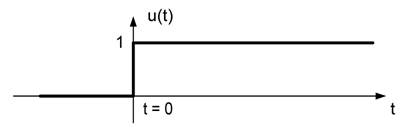
\includegraphics[width=6cm]{bilder/unitstep.png}
\end{minipage}


\subsection{Impulsfunktion - dirac delta function}
	\begin{minipage}{10cm}
		$\delta (t)=\begin{cases} 0 & t\ne 0\\\infty & t=0\end{cases} \qquad
		\text{und} \qquad \int\limits_{-\infty}^\infty \delta(t) \, \mathrm dt = 1 $\\
		$$\frac{du(t)}{dt}=\delta(t) \qquad
		\int\limits_{-\infty}^{\infty}\delta(t-t_0)f(t)dt=f(t_0)$$
	\end{minipage}
	\begin{minipage}{8cm}
		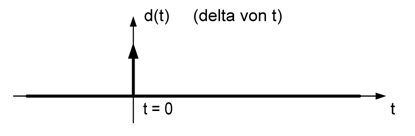
\includegraphics[width=6cm]{bilder/diracimpulse.png}
	\end{minipage}


\skriptsubsection{Impulsantwort}{25-2.2B}
Siehe Signale \& Systeme Zusammenfassung.\\
%$h(t) = T[\delta(t)] \qquad $


\skriptsubsection{Verzerrungen}{26}
\subsubsection{Amplitudenverzerrung}
Falls das Amplitudenspektrum $|H(\omega)|$ im gewünschten Frequenzband nicht konstant ist,
resultieren Amplitudenverzerrungen.

\subsubsection{Phasenverzerrung}
Falls das Phasenspektrum $\Theta_h (\omega)$ nicht linear von der Frequenz abhängig ist, resultieren
Phasenverzerrungen.\\



\skriptsubsection{Filter}{27}
\begin{multicols}{2}
\begin{center}
\begin{tabular}{|c|c|c|}
\hline
Tiefpass & Lowpass Filter & LPF \\
\hline
Hochpass & Heighpass Filter & HPF \\
\hline
Bandpass & Bandpass Filter & BPF \\
\hline
Bandsperre & Bandstop Filter & BSF \\
\hline
\end{tabular}
\end{center}
\columnbreak

\textbf{Ideale Filter} sind nicht realisierbar, da sie akausal sind.
\end{multicols}

\skriptsubsubsection{Bandbreite}{28}
\begin{minipage}{7cm}
	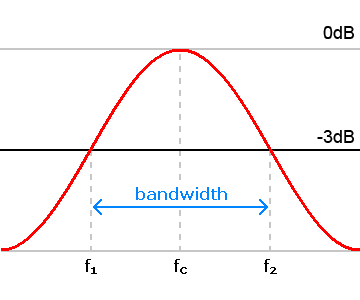
\includegraphics[width=6cm]{bilder/filter_bandbreite.png}
\end{minipage}
\begin{minipage}{11cm}
	Die Bandbreite ist nur für Tief- und Bandpassfilter definiert und bezieht sich auf das einseitige (reelle) Spektrum.
	\paragraph{LPF}	Die Bandbreite $W_B = 2 \pi B$ eines LPF entspricht der Frequenz, bei der $|H(\omega)|$ gegenüber $|H(0)|$ um $3 dB$ gedämpft ist
	\paragraph{BPF}	Filterbandbreite $W_B = 2 \pi B$ bei BPF entspricht der Differenz der (Kreis-) Frequenzen, bei denen Amplitudengang $|H(\omega)|$ gegenüber $|H(\omega_c)|$ um
	$3 dB$ gedämpft ist
\end{minipage}


\skriptsubsubsection{Quadraturfilter,
Hilberttransformation}{29}\label{lti_quadratur}\label{lti_hilbert}
Quadraturfilter und Hilberttransformation sind Allpassfilter mit
Phasendrehung um $-\frac{\pi}{2}\text{rad } (-90^\circ)$. Ein
Quadraturfilter ist technisch nur für einen beschränkten
Bandbreitenbereich realisierbar.
\[
H(\omega) = \begin{cases}
             	e^{-j \frac{\pi}{2}} & \omega > 0 \\
             	e^{j \frac{\pi}{2}} & \omega < 0
             \end{cases} =
-j \sgn(\omega)
\]

$\qquad \hat{X}(\omega) = H(\omega)X(\omega) = [-j \sgn(\omega)] X(\omega)$